\documentclass[]{article}
\usepackage[brazilian]{babel}
\usepackage[utf8]{inputenc}
\usepackage[T1]{fontenc}
\usepackage{graphics}
\usepackage{graphicx}
\usepackage{float}
\usepackage{listings}
\usepackage{color}

\definecolor{mygreen}{rgb}{0,0.6,0}
\definecolor{mygray}{rgb}{0.95,0.95,0.95}
\definecolor{mymauve}{rgb}{0.58,0,0.82}

\lstset{ %
	backgroundcolor=\color{mygray},
	basicstyle=\footnotesize,
	breakatwhitespace=true,
	breaklines=true,
	captionpos=b,
	commentstyle=\color{mygreen},
	frame=single,	                   % adds a frame around the code
	keepspaces=true,                 % keeps spaces in text, useful for keeping indentation of code (possibly needs columns=flexible)
	keywordstyle=\color{blue},       % keyword style
	language=python,                 % the language of the code
	morekeywords={*,...},            % if you want to add more keywords to the set
	numbers=left,                    % where to put the line-numbers; possible values are (none, left, right)
	numbersep=5pt,                   % how far the line-numbers are from the code
	numberstyle=\tiny\color{mygray}, % the style that is used for the line-numbers
	rulecolor=\color{black},         % if not set, the frame-color may be changed on line-breaks within not-black text (e.g. comments (green here))
	showspaces=false,                % show spaces everywhere adding particular underscores; it overrides 'showstringspaces'
	showstringspaces=false,          % underline spaces within strings only
	showtabs=false,                  % show tabs within strings adding particular underscores
	stepnumber=2,                    % the step between two line-numbers. If it's 1, each line will be numbered
	stringstyle=\color{mymauve},     % string literal style
	tabsize=2,	                   % sets default tabsize to 2 spaces
	title=\lstname                   % show the filename of files included with \lstinputlisting; also try caption instead of title
}


% Title Page
\title{Inteligência Artificial - MiniMax}
\author{ERZINGER Gabriel, TAETS Gabriel}


\begin{document}
\maketitle
	\section{Definição}
	\emph{Minimax} é um método usado na Teoria de Decisão e Teoria dos Jogos para minimizar a perda máxima possivel, ou seja, num ambiente em que as situações podem causar \emph{ganhos} ou \emph{percas} o algoritmo é utilizado para garantir que \textit{a maior perca que possa ocorrer} seja minimizada. \\
	
	O teorema foi demonstrado por Von Neumann, matemático considerado um dos pais da Teoria dos Jogos, em 1926.\\
	
	A teoria dos jogos foi desenvolvida com a finalidade de analisar situações competitivas que envolvem interesses conflitantes. Nestas situações, existem dois ou mais agentes com intensões diferentes cujas ações influenciam,  mas não determinam - \emph{completamente} - o resultado do jogo. \\
	
	Para estudar tal método, é necessário primeiro definir o que são jogos de soma zero. (Zero sum games). 
	
	\subsection{Zero Sum Games}
	Um jogo de soma zero é definido como um jogo em que quando um dos jogadores ganha, o outro perde, isso define uma \emph{soma zero}. Em tais jogos, a competitividade e estratégia é fator fundamental: não existe motivo para os jogadores colaborarem entre sí. Formalmente, num jogo de soma zero com dois jogadores o ganho de um jogador é a perca do outro.
	
	\subsection{Teorema Minimax}
	O Teorema Minimax de Von Neumann assegurava que para todos os jogos de duas pessoas e
	soma zero existia uma estratégia mista ótima para cada “jogador” e se eles as utilizassem
	teriam o mesmo resultado médio esperado, que seria o melhor ganho que cada “jogador”
	poderia esperar se o adversário jogasse racionalmente. \\
	
	Formalmente, o teorema minimax garante que, se atribuidos valores para cada conjunto de jogadas mistas, ie, um valor para cada sequência ou decisão tomada pelos jogadores A e B, um movimento que \emph{maximize} as chances do jogador A vencer, automaticamente \emph{minimiza} as chances do jogador B vencer. \\
	
	Dessa forma, temos - matematicamente - que:
	\textit{Sejam \textbf{X} e \textbf{Y} estratégias mistas para os jogadores \textbf{A e B}, seja também a matriz A a matriz de ganho do jogo, então:}
	
	$$max_x (min_y(X*A*Y)) = min_y (max_x(X*A*Y)) = v $$
	
	Onde v é chamado do \textit{valor do jogo} e X e Y são chamados de soluções. Além disso, também é provado que se existe mais de uma estratégia ótima, então existem infinitas estratégias ótimas. \cite{wolfram}
	
	
	
	\section{Aplicações e exemplos}
	
	O método minimax tem diversas aplicações em diversos campos de estudo - como a filosofia e a economia. Um dos exemplos mais simples e difundidos se trata da aplicação do minimax ao jogo da velha \emph{(tic-tac-toe.)}.
	\subsection{Jogo da velha}
	No famoso jogo da velha um jogador pode perder, empatar ou ganhar. Se o jogador A pode vencer com um movimento, esse é o seu melhor movimento.\\
	
	Se o jogador B identifica que um movimento levará a uma situação em que o adversário pode ganhar no próximo movimento, e que existe outro movimento que poderá levar a uma situação em que o adversário pode, no máximo, empatar, então, este último é o melhor movimento para ele.\\
	
    Após algumas rodadas, é fácil identificar qual é o melhor movimento. O algoritmo minimax ajuda a encontrar a melhor jogada, ao se caminhar pelas opções válidas, a partir do fim do jogo. A cada passo, assume-se que o jogador A está tentando maximizar as chances dele ganhar, enquanto na próxima rodada o jogador B está tentando minimizar as chances de isso acontecer (ao maximizar as chances de que ele próprio ganhe). \\
    \subsection{Competição de Empresas}
    Num artigo sobre teoria dos jogos, teorema minimax e equilibrio de Nash, a matemática Cristiene dos Santos utiliza o seguinte exemplo: \cite{artg} \\
    
    Duas redes de televisão competidoras, Mega e Plus, estão planejando levar ao ar programas
    de uma hora de duração para o mesmo horário. A rede Mega pode escolher um entre os
    programas A e B e a rede Plus um entre os programas C e D. Nenhuma delas sabe qual o
    programa a outra vai levar ao ar. Ambas contratam o mesmo instituto de pesquisa de opinião para lhes dar uma estimativa de como as possibilidades de transmitir os dois programas vão  dividir a audiência. \\
    
    A solução deste problema é encontrar a melhor estratégia, chamada de estratégia ótima de
    cada rede, de forma a maximizar a audiência. Disso resulta que ambos os “jogadores”
    tomarão decisões que podemos classificar como de anti-risco, ou seja, aquelas que renunciam
    a alguns ganhos possíveis para evitarem incorrer em perdas desnecessárias. Ao generalizar
    esta análise, conclui-se que \textbf{o decisor racional procurará um modo de atuação que lhe dê o
    melhor ganho possível na pior situação, ou seja, o melhor ganho admitindo que o oponente
    fará o melhor contra movimento}. \\
	
\section{Algoritmo}

\subsection{Metodologia}
	O algoritmo será implementado em \emph{Python} seguindo o seguinte raciocinio: \cite{gfg}\\
	
	Considerando um jogo qualquer que possui \emph{estados} que são alcançados após uma \emph{sequência de movimentos} realizadas pelos jogadores A e B, cada estado do jogo irá possuir um valor associado a ele. Em um dado estado, se o jogador A possui a vantagem, este estado tera um valor positivo. Caso contrário, o estado terá um valor negativo. Neste cenário, o jogador A tenta maximizar os valores, enquanto o jogador B tentará minimiza-los. \\
	
	Estes valores são calculados através de alguma heuristica que é única para cada tipo de jogo ou situação.\\
	
	Considerando um jogo com 4 estados finais possíveis representados numa árvore binária como a da figura abaixo, onde o primeiro jogador a jogar tem o objetivo de maximizar o resultado.
	
	\begin{figure}[H]
	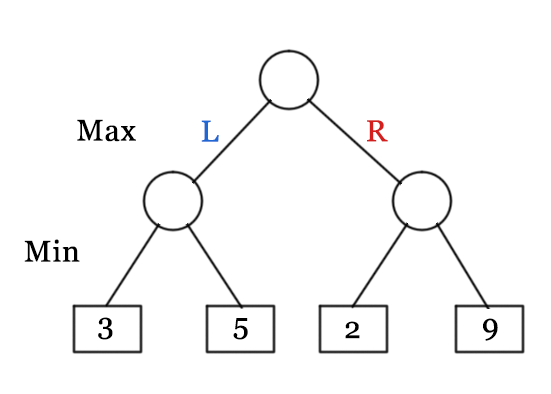
\includegraphics[width=\linewidth]{gtt.png}
	\caption{Arvore de Estados \cite{gfg}}
	\label{fig:arvore1}
	\end{figure}

	O algoritmo será implementado através de um \textit{Backtrac}, dessa forma, ele irá testar todos os movimentos possíveis e retornar o maior ganho. Os movimentos, considerando que o jogador B jogue de forma ótima são:
	\begin{itemize}
		\item Jogador A escolhe ir para a esquerda: Em seguida, o jogador B escolhe 3.
		\item Jogador A escolhe ir para a direita: Em seguida, o jogador B escolhe 2.
	\end{itemize}
	Dessa forma, o movimento ótimo para o jogador A é ir para a esquerda, uma vez que este movimento irá \emph{minimizar a sua perca}, ie, entre os dois valores finais prováveis [2 e 3], ele escolherá o maior. Isto pode ser representado pela segunda árvore de estados:
	\begin{figure}[H]
	   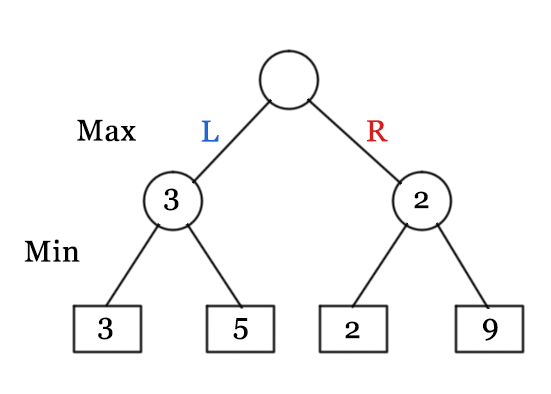
\includegraphics[width=\linewidth]{gtt2.png}
	   \caption{Arvore de Estados Final\cite{gfg}}
	   \label{fig:arvore2}
	\end{figure}
	
	
	
\subsection{Implementação}
 Abaixo temos uma implementação em \emph{python} do minimax para o jogo descrito previamente.
	\begin{lstlisting}[]
	#Funcao minimax para o jogo Maximizer x Minimizer que define a pontuacao maxima que o Maximizer pode obter comecando se ambos jogarem de forma otima.
	
	import math
	
	def minimax(profundidade, indice, jogador, placar, h):
	if (profundidade == h): # Se a profundidade chegou ao fim
		return placar[indice] # Retorna o placar deste indice	
	
	#Se eh o jogador A ( maximizer )
	#Maximo entre ir pra Dir/Esq
	if(jogador == 1): 
		return max(minimax(profundidade+1, indice*2, 0, placar, h),  
	minimax(profundidade+1, indice*2 + 1, 0, placar, h)) 
	
	 #Se eh o jogador B ( minimizer ) #Mininmo entre ir pra Dir/Esq
	else:
		return min(minimax(profundidade+1, indice*2, 1, placar, h), 
	minimax(profundidade+1, indice*2 + 1, 1, placar, h))
	
	
	
	
	placar = [3, 5, 2, 9, 12, 5, 23, 23] # Arvore
	n = 8 # Numero de elementos
	altura = (math.log(n)/math.log(2))
	res = minimax(0,0,1,placar, altura)
	s = 'O melhor valor alcancado por A eh ' + str(res)
	print(s)
	
	\end{lstlisting}
	
\begin{thebibliography}{1}
	\bibitem{artg} COSTA, Cristiene dos Santos - \textit{TEORIA DOS JOGOS E A RELAÇÃO ENTRE O “TEOREMA MINIMAX” DE JOHN VON NEUMANN E O “EQUILÍBRIO DE NASH” DE JOHN NASH} <https://repositorio.ucb.br/jspui/bitstream/10869/1549/1/Cristiene\%20dos\%
	20Santos\%20Costa.pdf> Acesso em 01/Setembro/2017.
	
	\bibitem{wolfram} Weisstein, Eric W. "Minimax Theorem." From MathWorld--A Wolfram Web Resource. http://mathworld.wolfram.com/MinimaxTheorem.html
	
	\bibitem{gfg} Minimax Algorithm in Game Theory | Set 1. From GeeksForGeeks  http://www.geeksforgeeks.org/minimax-algorithm-in-game-theory-set-1-introduction/.
	
\end{thebibliography}	 
	
\end{document}          
